\chapter{Titraties met pH en geleidbaarheid}\label{ch:g12:ph-conductivity-titrations}

Op een fles wijnazijn staat ``6 \% zuurgraad'': zes gram ethaanzuur in
elke honderd gram azijn. Ethaanzuur en zijn geconjugeerde base zijn
allebei kleurloos, en permanganaat helpt hier niet. Maar een \omterm{def:g9:acids-bases-ph:ph-paper}{pH-meter} in
de azijn, of een cel die meet hoe goed hij geleidt, volgt de reactie met
een base druppel voor druppel, en de vorm van de kromme laat precies zien
waar het \omterm{def:g11:titration:equivalence}{equivalentiepunt} ligt. Tien minuten aan de labtafel, en het
etiket is gecontroleerd.

\begin{recall}
Een \omterm{def:g11:titration:titration}{titratie}, haar \omterm{def:g11:titration:equivalence}{equivalentiepunt} en \omterm{def:g11:titration:equivalence}{equivalentievolume}
(\cref{ch:g11:titration}); \omterm{def:g12:ka-and-pka:ka}{zuurconstanten} (\cref{ch:g12:ka-and-pka});
de betrekking van Henderson en indicatoren
(\cref{ch:g12:buffers-predominance}); oplossingen van \omterm{def:g9:ions:ion}{ionen} geleiden
elektriciteit (\cref{ch:g9:ions}).
\end{recall}

\begin{omfigure}
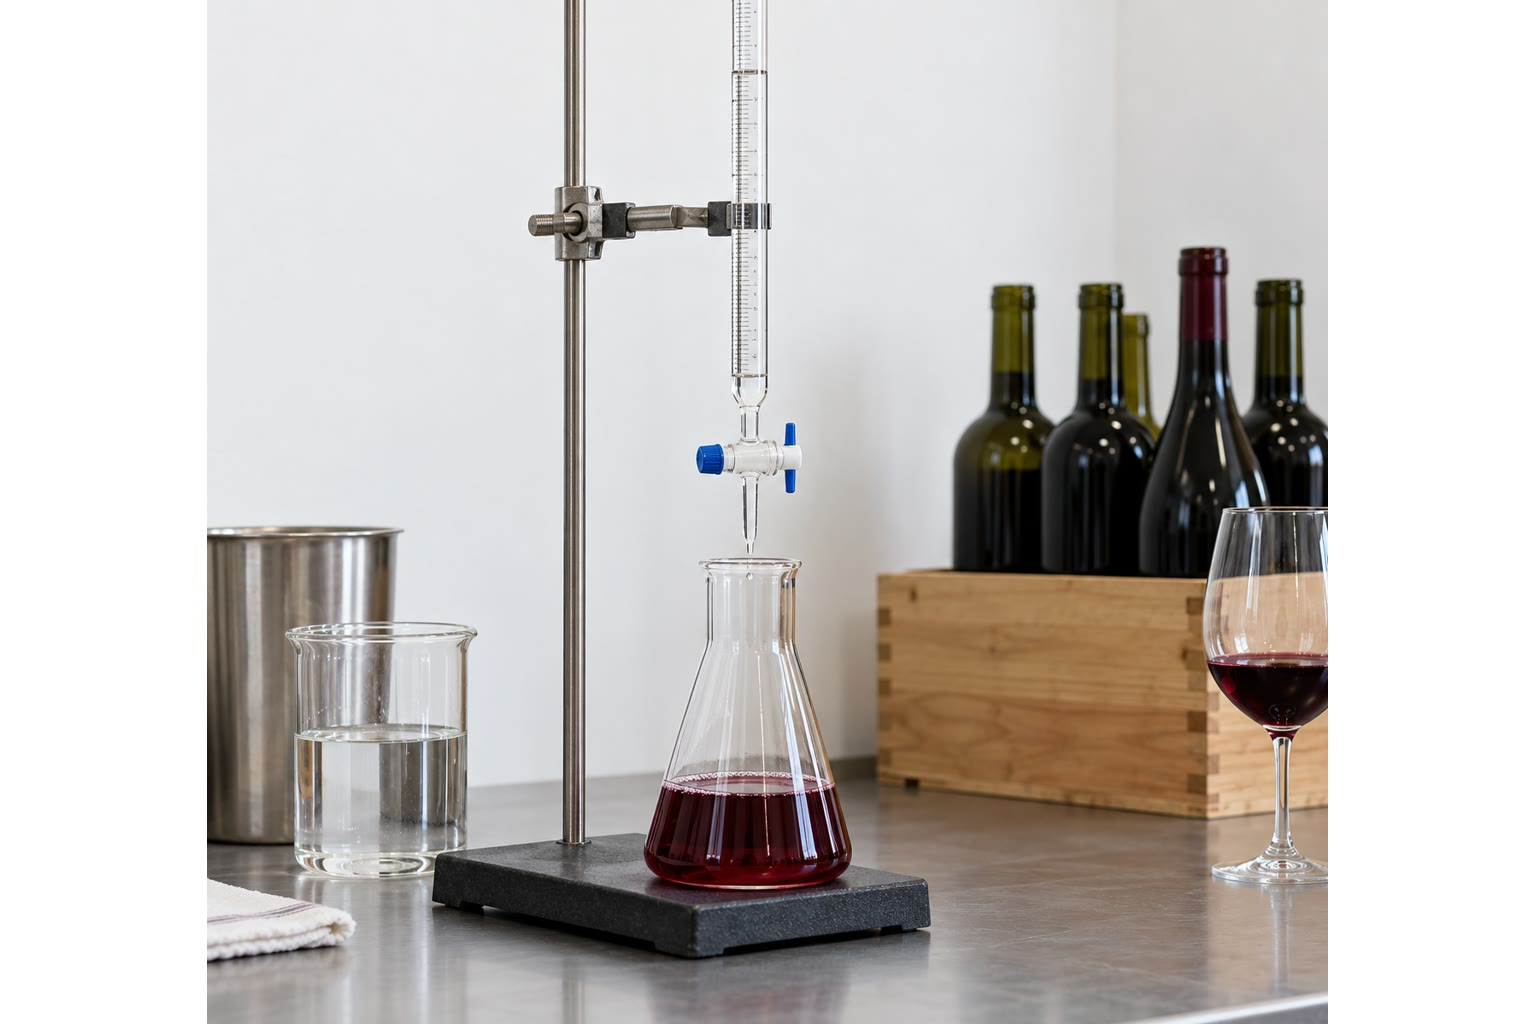
\includegraphics[width=0.45\linewidth]{images/book1/ai/g12-wine-lab.jpg}

{\small De titratietafel van een wijnmaker.}
\end{omfigure}

\section{De pH-metrische titratie}

\begin{definition}[pH-metrische titratie, halfequivalentiepunt]\label{def:g12:ph-conductivity-titrations:ph-metric}
Bij een \emph{pH-metrische titratie}\index{pH-metrische titratie} wordt
na elke toevoeging van \omterm{def:g11:titration:titration}{titrant} de \omterm{def:g9:acids-bases-ph:ph}{pH} van de \omterm{def:g11:titration:titration}{getitreerde oplossing} gemeten,
en wordt de kromme van de \omterm{def:g9:acids-bases-ph:ph}{pH} tegen het toegevoegde volume getekend. Het
\emph{halfequivalentiepunt}\index{halfequivalentiepunt}
is het punt waarop de helft van het \omterm{def:g11:titration:equivalence}{equivalentievolume} is toegevoegd.
\end{definition}

\begin{omfigure}
\begin{tikzpicture}[font=\small, scale=0.65]
  \pic[transform shape] at (0,0) {stand={6.3}{2.0}};
  \pic[transform shape] at (2.0,0.68) {stirrer};
  \pic[transform shape] at (2.0,0.68) {beaker={0.45}{omWater}};
  \pic[transform shape] at (2.0,2.9) {burette={0.8}{omWater}};
  \pic[transform shape] (pr) at (2.6,0.95) {probe};
  \pic[transform shape] (m) at (6.4,3.4) {meter={pH}};
  \draw[black!70, thick] (pr-top) .. controls +(0,1.0) and +(0,-1.2) .. (m-a);
  \draw[omProp, thick, <-] (2.35,7.2) -- (4.3,7.6) node[right, text=black] {buret: NaOH};
  \draw[omProp, thick, <-] (1.4,1.1) -- (-1.4,1.6) node[left, text=black, align=right] {te titreren zuur};
  \draw[omProp, thick, <-] (2.75,2.4) -- (4.3,2.0) node[right, text=black] {pH-elektrode};
\end{tikzpicture}

{\small Een \omterm{def:g12:ph-conductivity-titrations:ph-metric}{pH-metrische titratie}: de elektrode hangt in de geroerde
oplossing, de meter toont na elke toevoeging de \omterm{def:g9:acids-bases-ph:ph}{pH}.}
\end{omfigure}

\begin{inthelab}[Een pH-meter ijken]
Voor gebruik wordt de elektrode afgespoeld met gedestilleerd water en in
twee \omterm{def:g12:buffers-predominance:buffer}{bufferoplossingen} met een bekende \omterm{def:g9:acids-bases-ph:ph}{pH} gedompeld, meestal 7.0 en 4.0
(of 10.0): de meter wordt zo ingesteld dat hij hun waarden aangeeft.
Tussen twee oplossingen wordt de elektrode afgespoeld en voorzichtig
drooggedept, nooit afgeveegd; ze wordt bewaard met een natte punt.
\end{inthelab}

\begin{omfigure}
\begin{minipage}{0.49\linewidth}
\begin{tikzpicture}
\begin{axis}[width=\linewidth, height=6cm, xmin=0, xmax=30, ymin=0, ymax=14,
    xlabel={$V_{\text{NaOH}}$ (\si{mL})}, ylabel={pH}, axis lines*=left,
    ymajorgrids, grid style={gray!20}, tick label style={font=\scriptsize},
    label style={font=\small}, title={\small \ce{HCl} met \ce{NaOH}},
    title style={yshift=-4pt}]
  \addplot[very thick, omDef] table[x=V, y=pH] {figdata/out/grade-12-ph-conductivity-titrations-a.dat};
  \addplot[thick, omProp, densely dotted] table[x=V, y expr=\thisrow{dpH}/4]
    {figdata/out/grade-12-ph-conductivity-titrations-a.dat};
  \addplot[dashed, black!60] coordinates {(20,0) (20,7)};
  \node[font=\scriptsize, anchor=north west] at (axis cs:20.3,6.5) {$V_E = 20.0$};
\end{axis}
\end{tikzpicture}
\end{minipage}\hfill
\begin{minipage}{0.49\linewidth}
\begin{tikzpicture}
\begin{axis}[width=\linewidth, height=6cm, xmin=0, xmax=16, ymin=0, ymax=14,
    xlabel={$V_{\text{NaOH}}$ (\si{mL})}, ylabel={pH}, axis lines*=left,
    ymajorgrids, grid style={gray!20}, tick label style={font=\scriptsize},
    label style={font=\small}, title={\small \ce{CH3COOH} met \ce{NaOH}},
    title style={yshift=-4pt}]
  \addplot[very thick, omDef] table[x=V, y=pH] {figdata/out/grade-12-ph-conductivity-titrations-b.dat};
  \addplot[thick, omProp, densely dotted] table[x=V, y expr=\thisrow{dpH}/4]
    {figdata/out/grade-12-ph-conductivity-titrations-b.dat};
  \addplot[dashed, black!60] coordinates {(10.1,0) (10.1,8.7)};
  \addplot[dashed, black!60] coordinates {(0,4.76) (5.05,4.76) (5.05,0)};
  \node[font=\scriptsize, anchor=south west] at (axis cs:0.2,4.8) {$pK_a = 4.76$};
  \node[font=\scriptsize, anchor=north west] at (axis cs:10.4,3.0) {$V_E = 10.1$};
\end{axis}
\end{tikzpicture}
\end{minipage}

{\small Berekende pH-krommen (blauw) en hun afgeleide $d\mathrm{pH}/dV$
(oranje, gestippeld, gedeeld door 4). Links: \qty{20.0}{mL} zoutzuur van
\qty{0.100}{mol/L}; \omterm{def:g11:titration:equivalence}{equivalentiepunt} bij \omterm{def:g9:acids-bases-ph:ph}{pH} 7.00. Rechts: \qty{10.0}{mL}
verdunde azijn; bij het \omterm{def:g12:ph-conductivity-titrations:ph-metric}{halfequivalentiepunt} is de \omterm{def:g9:acids-bases-ph:ph}{pH} gelijk aan de
$pK_a$, en het \omterm{def:g11:titration:equivalence}{equivalentiepunt} ligt bij een basische \omterm{def:g9:acids-bases-ph:ph}{pH}.}
\end{omfigure}


\begin{method}[De afgeleidemethode]\label{met:g12:ph-conductivity-titrations:derivative}
Bereken tussen opeenvolgende metingen de helling
$\Delta\mathrm{pH}/\Delta V$, en zet die uit tegen $V$ (een spreadsheet of
een rekenmachine doet dat). Het \omterm{def:g11:titration:equivalence}{equivalentievolume} ligt waar deze helling
het grootst is: de piek van de afgeleide kromme.
\end{method}

\begin{method}[De raaklijnenmethode]\label{met:g12:ph-conductivity-titrations:tangent}
\begin{enumerate}
  \item Teken twee evenwijdige raaklijnen aan de kromme, een vóór en een
        na de sprong, aan weerszijden ervan.
  \item Teken de evenwijdige lijn halverwege daartussen.
  \item Waar die de kromme snijdt, ligt het \omterm{def:g11:titration:equivalence}{equivalentiepunt}: lees $V_E$
        af (en de \omterm{def:g9:acids-bases-ph:ph}{pH} bij het \omterm{def:g11:titration:equivalence}{equivalentiepunt}).
\end{enumerate}
\end{method}

\begin{proposition}[Bij het halfequivalentiepunt is $\mathrm{pH} = pK_a$]\label{prop:g12:ph-conductivity-titrations:half}
Bij de \omterm{def:g11:titration:titration}{titratie} van een \omterm{def:g12:ka-and-pka:strong-acid}{zwak zuur} \ce{HA} met een \omterm{def:g12:ka-and-pka:strong-acid}{sterke base} geldt bij
het \omterm{def:g12:ph-conductivity-titrations:ph-metric}{halfequivalentiepunt} $\mathrm{pH} = pK_a$.
\end{proposition}

\begin{proof}
De reactie \ce{HA + OH- -> A- + H2O} is aflopend. Bij het
\omterm{def:g12:ph-conductivity-titrations:ph-metric}{halfequivalentiepunt} is de helft van het zuur omgezet in \ce{A-}:
$[\ce{A-}] = [\ce{HA}]$, en de betrekking van Henderson geeft
$\mathrm{pH} = pK_a + \log 1 = pK_a$.
\end{proof}

\begin{remark}[Een indicator kiezen met de kromme]\label{rem:g12:ph-conductivity-titrations:indicator}
% ledger: ind:BBT, ind:phenolphthalein
De indicator moet binnen de sprong omslaan. Bij zoutzuur loopt de sprong
van ongeveer \omterm{def:g9:acids-bases-ph:ph}{pH} 4 tot 10 en passen veel indicatoren, broomthymolblauw het
best; bij ethaanzuur is de sprong korter en basisch, rond 7 tot 11:
fenolftaleïne (8.0--10.0) past, broomthymolblauw zou te vroeg
omslaan.
\end{remark}

\section{Geleidbaarheid en conductometrische titraties}

\begin{definition}[Geleidbaarheid, molaire ionengeleidbaarheid]\label{def:g12:ph-conductivity-titrations:conductivity}
De \emph{geleidbaarheid}\index{geleidbaarheid} $\sigma$ van een oplossing
meet hoe goed ze elektriciteit geleidt; je leest haar af op een
geleidbaarheidsmeter, in \si{mS/cm} (of \si{S/m}). Elk \omterm{def:g9:ions:ion}{ion} $i$ draagt eraan
bij in verhouding tot zijn concentratie, met een coëfficiënt $\lambda_i$,
zijn \emph{molaire ionengeleidbaarheid}\index{molaire ionengeleidbaarheid}.
\end{definition}

\begin{proposition}[De wet van Kohlrausch]\label{prop:g12:ph-conductivity-titrations:kohlrausch}
% ledger: lam:H+, lam:OH-, lam:Na+, lam:Cl-
Voor een verdunde oplossing geldt $\sigma = \sum_i \lambda_i [X_i]$. Bij
\qty{25}{\celsius}, in \si{S.cm^2/mol}: \ce{H3O+} 349.8, \ce{OH-} 198.3,
\ce{Cl-} 76.2, \ce{Na+} 50.3. De oxonium- en \omterm{def:g9:ions:ion}{hydroxide-ionen} geleiden veel
beter dan alle andere \omterm{def:g9:ions:ion}{ionen}.
\end{proposition}

\begin{proof}
Aangenomen (deel voor het eerste universiteitsjaar). De waarden van
\ce{Cl-} en \ce{Na+} komen uit de gemeten geleidbaarheden van oplossingen
van zoutzuur en natriumchloride, waarvan die van \ce{H3O+} wordt
afgetrokken.
\end{proof}

\begin{definition}[Conductometrische titratie]\label{def:g12:ph-conductivity-titrations:conductimetric}
Bij een \emph{conductometrische titratie}\index{conductometrische titratie}
wordt na elke toevoeging van \omterm{def:g11:titration:titration}{titrant} de \omterm{def:g12:ph-conductivity-titrations:conductivity}{geleidbaarheid} gemeten.
De \omterm{def:g11:titration:titration}{getitreerde oplossing} wordt verdund in een groot volume water, zodat
het toegevoegde volume het nauwelijks verandert: de punten liggen dan op
rechte lijnen, die bij het \omterm{def:g11:titration:equivalence}{equivalentiepunt} van helling veranderen.
\end{definition}

\begin{omfigure}
\begin{minipage}{0.4\linewidth}\centering
\begin{tikzpicture}[font=\small, scale=0.75]
  \pic[transform shape] at (0,0) {beaker={0.6}{omWater}};
  \pic[transform shape] (cc) at (0.2,0.2) {condcell};
  \pic[transform shape] (m) at (2.6,3.4) {meter={mS/cm}};
  \draw[black!70, thick] (cc-top) .. controls +(0,0.8) and +(0,-1) .. (m-a);
  \node[anchor=north, align=center] at (0.6,-0.15) {geleidbaarheidscel\\ in de oplossing};
\end{tikzpicture}
\end{minipage}\hfill
\begin{minipage}{0.56\linewidth}
\begin{tikzpicture}
\begin{axis}[width=\linewidth, height=5.4cm, xmin=0, xmax=20, ymin=0,
    ymax=4.6, xlabel={$V_{\text{NaOH}}$ (\si{mL})}, ylabel={$\sigma$ (\si{mS/cm})},
    axis lines*=left, ymajorgrids, grid style={gray!20},
    tick label style={font=\scriptsize}, label style={font=\small}]
  \addplot[only marks, mark=*, mark size=1.4pt, omDef] table[x=V, y=sigma]
    {figdata/out/grade-12-ph-conductivity-titrations-c.dat};
  \addplot[dashed, black!60] coordinates {(10,0) (10,4.6)};
  \node[font=\scriptsize, anchor=south west] at (axis cs:10.3,0.2) {$V_E = 10.0$};
\end{axis}
\end{tikzpicture}
\end{minipage}

{\small Links: een geleidbaarheidscel. Rechts: \qty{100}{mL} zoutzuur van
\qty{0.0100}{mol/L} getitreerd met natronloog van
\qty{0.100}{mol/L} (berekend met de wet van Kohlrausch). De
\omterm{def:g12:ph-conductivity-titrations:conductivity}{geleidbaarheid} daalt en stijgt dan weer: twee rechte lijnen die elkaar bij
het \omterm{def:g11:titration:equivalence}{equivalentiepunt} ontmoeten.}
\end{omfigure}

\begin{example}[De twee lijnen aflezen]\label{ex:g12:ph-conductivity-titrations:lines}
Vóór het \omterm{def:g11:titration:equivalence}{equivalentiepunt} haalt elk toegevoegd \ce{OH-} een \ce{H3O+} weg
($\lambda = 349.8$) en brengt het een \ce{Na+} binnen ($\lambda = 50.3$):
de \omterm{def:g12:ph-conductivity-titrations:conductivity}{geleidbaarheid} daalt sterk. Na het \omterm{def:g11:titration:equivalence}{equivalentiepunt} hopen \ce{Na+} en
\ce{OH-} ($\lambda = 198.3$) zich gewoon op: ze stijgt. De twee lijnen
ontmoeten elkaar bij
$V_E = \qty{10.0}{mL}$, dus het zuur was
$0.100 \times 10.0 / 100 = \qty{0.0100}{mol/L}$.
\end{example}

\begin{method}[Het equivalentiepunt uit een conductometrische titratie]\label{met:g12:ph-conductivity-titrations:two-lines}
Trek de best passende rechte lijn door de punten vóór het
\omterm{def:g11:titration:equivalence}{equivalentiepunt} en de best passende lijn door de punten erna; lees $V_E$
af bij hun snijpunt. Punten vlak bij het \omterm{def:g11:titration:equivalence}{equivalentiepunt}, waar de lijnen
buigen, laat je weg.
\end{method}

\begin{remark}[Welke methode wanneer]\label{rem:g12:ph-conductivity-titrations:which}
Een gekleurde indicator is het snelst als er een geschikte bestaat. Een
\omterm{def:g12:ph-conductivity-titrations:ph-metric}{pH-metrische titratie} geeft ook de $pK_a$ van een \omterm{def:g12:ka-and-pka:strong-acid}{zwak zuur}, en werkt met
gekleurde of troebele oplossingen. Een \omterm{def:g12:ph-conductivity-titrations:conductimetric}{conductometrische titratie} heeft
helemaal geen pH-sprong nodig: ze werkt voor heel zwakke of heel verdunde
zuren, en voor \omterm{def:g9:ions:precipitate}{neerslagreacties}, zolang de \omterm{def:g9:ions:ion}{ionen} veranderen.
\end{remark}

\begin{safety}{\ghs[0.82cm]{GHS05}\ghs[0.82cm]{GHS07}}
% ledger: ghs:NaOH
Oplossingen van natriumhydroxide branden huid en ogen, in de ogen zelfs
als ze verdund zijn: draag de hele tijd een veiligheidsbril, en spoel
elke spat meteen af met veel water.
\end{safety}

\section{Oefeningen}


\begin{exercise}[$\star$]\label{exo:g12:ph-conductivity-titrations:1}
Lees het \omterm{def:g11:titration:equivalence}{equivalentievolume} af op de kromme van zoutzuur dat getitreerd
wordt met natronloog van \qty{0.100}{mol/L}, en leid de concentratie van
de \qty{20.0}{mL} zuur af.
\end{exercise}

\begin{exercise}[$\star$]\label{exo:g12:ph-conductivity-titrations:2}
Een \omterm{def:g12:ka-and-pka:strong-acid}{zwak zuur} wordt getitreerd met natronloog; $V_E = \qty{12.0}{mL}$.
Bij \qty{6.0}{mL} is de \omterm{def:g9:acids-bases-ph:ph}{pH} 3.75. Geef de $pK_a$ van het zuur. Welk zuur
van de $pK_a$-schaal zou het kunnen zijn?
\end{exercise}

\begin{exercise}[$\star$]\label{exo:g12:ph-conductivity-titrations:3}
Welke indicator zou je kiezen voor de \omterm{def:g11:titration:titration}{titratie} van ethaanzuur met
natronloog? Waarom niet methylrood?
\end{exercise}

\begin{exercise}[$\star$]\label{exo:g12:ph-conductivity-titrations:4}
Waarom moet een \omterm{def:g9:acids-bases-ph:ph-paper}{pH-meter} voor gebruik geijkt worden? Waarmee?
\end{exercise}

\begin{exercise}[$\star$]\label{exo:g12:ph-conductivity-titrations:5}
Zet met de molaire ionengeleidbaarheden de \omterm{def:g9:ions:ion}{ionen} \ce{H3O+}, \ce{OH-},
\ce{Na+}, \ce{Cl-} op volgorde van de beste geleider naar de slechtste.
\end{exercise}

\begin{exercise}[$\star\star$]\label{exo:g12:ph-conductivity-titrations:6}
Voor \qty{20.0}{mL} van een oplossing van ethaanzuur is \qty{14.6}{mL}
natronloog van \qty{0.050}{mol/L} nodig. Bereken de concentratie ervan.
\end{exercise}

\begin{exercise}[$\star\star$]\label{exo:g12:ph-conductivity-titrations:7}
Vlak bij het \omterm{def:g11:titration:equivalence}{equivalentiepunt} zijn de aflezingen: \qty{9.6}{mL}, \omterm{def:g9:acids-bases-ph:ph}{pH} 5.7;
\qty{9.8}{mL}, 6.1; \qty{10.0}{mL}, 7.0; \qty{10.2}{mL}, 10.5;
\qty{10.4}{mL}, 11.0. Bereken $\Delta\mathrm{pH}/\Delta V$ tussen
opeenvolgende punten en bepaal $V_E$.
\end{exercise}

\begin{exercise}[$\star\star$]\label{exo:g12:ph-conductivity-titrations:8}
Verklaar bij de \omterm{def:g12:ph-conductivity-titrations:conductimetric}{conductometrische titratie} van zoutzuur het teken van de
helling vóór en na het \omterm{def:g11:titration:equivalence}{equivalentiepunt}, met de \omterm{def:g9:ions:ion}{ionen} die aanwezig zijn.
\end{exercise}

\begin{exercise}[$\star\star$]\label{exo:g12:ph-conductivity-titrations:9}
Schets de conductometrische kromme van ethaanzuur dat getitreerd wordt met
natronloog. Waarom stijgt de \omterm{def:g12:ph-conductivity-titrations:conductivity}{geleidbaarheid} al vóór het \omterm{def:g11:titration:equivalence}{equivalentiepunt}?
\end{exercise}

\begin{exercise}[$\star\star$]\label{exo:g12:ph-conductivity-titrations:10}
Lees op de berekende kromme van de verdunde azijn de \omterm{def:g9:acids-bases-ph:ph}{pH} af aan het begin,
bij het \omterm{def:g12:ph-conductivity-titrations:ph-metric}{halfequivalentiepunt} en bij het \omterm{def:g11:titration:equivalence}{equivalentiepunt}. Waarom is de
\omterm{def:g9:acids-bases-ph:ph}{begin-pH} veel hoger dan die van zoutzuur van dezelfde concentratie?
\end{exercise}

\begin{exercise}[$\star\star$]\label{exo:g12:ph-conductivity-titrations:11}
Waarom wordt de \omterm{def:g11:titration:titration}{getitreerde oplossing} vóór een \omterm{def:g12:ph-conductivity-titrations:conductimetric}{conductometrische titratie}
verdund in een groot volume water?
\end{exercise}

\begin{exercise}[$\star\star\star$]\label{exo:g12:ph-conductivity-titrations:12}
Een oplossing bevat zowel zoutzuur als ethaanzuur. Ze wordt getitreerd met
natronloog terwijl de \omterm{def:g9:acids-bases-ph:ph}{pH} gemeten wordt. Leg uit waarom de kromme twee
sprongen vertoont, en wat elk \omterm{def:g11:titration:equivalence}{equivalentievolume} meet.
\end{exercise}

\begin{exercise}[$\star\star\star$]\label{exo:g12:ph-conductivity-titrations:13}
Bereken de \omterm{def:g12:ph-conductivity-titrations:conductivity}{geleidbaarheid} aan het begin van de \omterm{def:g12:ph-conductivity-titrations:conductimetric}{conductometrische titratie}
van het hoofdstuk (zoutzuur van \qty{0.0100}{mol/L}) en bij het
\omterm{def:g11:titration:equivalence}{equivalentiepunt} (\qty{110}{mL} oplossing van natriumchloride).
Vergelijk met de figuur.
\end{exercise}

\begin{exercise}[$\star\star\star$]\label{exo:g12:ph-conductivity-titrations:14}
Een slecht geijkte \omterm{def:g9:acids-bases-ph:ph-paper}{pH-meter} geeft elke \omterm{def:g9:acids-bases-ph:ph}{pH} 0.2 te hoog aan. Welke fout
veroorzaakt dat in het \omterm{def:g11:titration:equivalence}{equivalentievolume} van een \omterm{def:g12:ph-conductivity-titrations:ph-metric}{pH-metrische titratie}?
En in de $pK_a$ die bij het \omterm{def:g12:ph-conductivity-titrations:ph-metric}{halfequivalentiepunt} wordt afgelezen?
\end{exercise}

\begin{exercise}[$\star\star\star$]\label{exo:g12:ph-conductivity-titrations:15}
Waarom kan een \omterm{def:g12:ph-conductivity-titrations:conductimetric}{conductometrische titratie} de reactie van zilverionen met
\omterm{def:g9:ions:ion}{chloride-ionen}, \ce{Ag+ + Cl- -> AgCl(s)}, volgen, en een \omterm{def:g12:ph-conductivity-titrations:ph-metric}{pH-metrische
titratie} niet? Beschrijf de verwachte kromme als zilvernitraat aan
natriumchloride wordt toegevoegd (neem voor $\lambda$ van \ce{NO3-} een
waarde dicht bij die van \ce{Cl-}).
\end{exercise}

\section{Probleem: Is de azijn 6\,\%?}

\begin{problem}[{Weekendprobleem --- bevat een azijn met ``6 \% zuurgraad''
op het etiket echt zes gram ethaanzuur per honderd gram?}]
\label{pb:g12:ph-conductivity-titrations:1}
% ledger: pka:ethanoic, ind:phenolphthalein, lam:OH-, lam:Na+, aw:C, aw:H, aw:O
Een azijn met ``6 \% zuurgraad'' op het etiket wordt gecontroleerd.
\qty{100.0}{mL} ervan wordt gewogen: \qty{101}{g}. De azijn wordt tien
keer verdund, en daarna wordt \qty{10.0}{mL} van de verdunde oplossing
getitreerd met natronloog van \qty{0.100}{mol/L}, met een \omterm{def:g9:acids-bases-ph:ph-paper}{pH-meter}; de
berekende kromme van het hoofdstuk (rechts) komt overeen met de metingen.

\medskip
\noindent\textbf{Deel I --- Het monster klaarmaken.}
\begin{enumerate}
  \item Wat betekent ``6 \% zuurgraad''?
  \item Welke massa ethaanzuur bevat \qty{100.0}{mL} azijn als het
        etiket klopt? Welke \omterm{def:g10:concentration-and-dilution:molar-concentration}{molaire concentratie} is dat?
  \item Waarom wordt de azijn vóór de \omterm{def:g11:titration:titration}{titratie} verdund?
  \item Met welk glaswerk verdun je hem tien keer?
\end{enumerate}

\medskip
\noindent\textbf{Deel II --- De \omterm{def:g12:ph-conductivity-titrations:ph-metric}{pH-metrische titratie}.}
\begin{enumerate}[resume]
  \item Schrijf de vergelijking van de titratiereactie op.
  \item Lees het \omterm{def:g11:titration:equivalence}{equivalentievolume} af op de kromme.
  \item Bereken de concentratie van de verdunde azijn.
  \item Leid daaruit die van de azijn af.
  \item Lees de \omterm{def:g9:acids-bases-ph:ph}{pH} af bij het \omterm{def:g12:ph-conductivity-titrations:ph-metric}{halfequivalentiepunt}. Wat levert die op?
  \item Waarom ligt de \omterm{def:g9:acids-bases-ph:ph}{pH} bij het \omterm{def:g11:titration:equivalence}{equivalentiepunt} boven 7?
  \item Welke indicator had hetzelfde resultaat gegeven?
\end{enumerate}

\medskip
\noindent\textbf{Deel III --- Een conductometrische controle.}
\begin{enumerate}[resume]
  \item De \omterm{def:g11:titration:titration}{titratie} wordt herhaald met een geleidbaarheidscel, met het
        monster verdund in \qty{200}{mL} water. Welke \omterm{def:g9:ions:ion}{ionen} verschijnen er
        vóór het \omterm{def:g11:titration:equivalence}{equivalentiepunt} in de oplossing?
  \item Waarom stijgt de \omterm{def:g12:ph-conductivity-titrations:conductivity}{geleidbaarheid} vóór het \omterm{def:g11:titration:equivalence}{equivalentiepunt} maar
        langzaam?
  \item Waarom stijgt ze daarna sneller?
  \item Waarom is de \omterm{def:g12:ph-conductivity-titrations:conductivity}{geleidbaarheid} aan het begin heel laag?
  \item Waar zouden de twee lijnen elkaar moeten ontmoeten?
\end{enumerate}

\medskip
\noindent\textbf{Deel IV --- Het oordeel.}
\begin{enumerate}[resume]
  \item Bereken de \omterm{def:g10:concentration-and-dilution:mass-concentration}{massaconcentratie} ethaanzuur in de azijn.
  \item Bereken de massa ethaanzuur in \qty{100.0}{mL} azijn.
  \item Leid daaruit de massa ethaanzuur per \qty{100}{g} azijn af.
  \item Geef het eindantwoord: wat is de zuurgraad van de azijn?
\end{enumerate}
\end{problem}
